\documentclass{beamer}

\usepackage{../../../latex_style/beamerthemeExecushares}
\usepackage{../../../latex_style/notations}

\title{Session 6: Eigenvalues, eigenvectors \& Markov chains}
\subtitle{Optimization and Computational Linear Algebra for Data Science}
\author{Léo Miolane}
\date{}

\setcounter{showSlideNumbers}{1}

\begin{document}
\setcounter{showProgressBar}{0}
\setcounter{showSlideNumbers}{0}

\frame{\titlepage}

\begin{frame}
	\frametitle{Contents}
	\begin{enumerate}
		\item Orthogonal matrices
		\item Eigenvalues \& eigenvectors
		\item Properties of eigenvalues and eigenvectors
		\item Markov chains
	\end{enumerate}
\end{frame}


\setcounter{framenumber}{0}
\setcounter{showSlideNumbers}{1}

\section{Orthogonal matrices}

\begin{frame}[t]{Orthogonal matrices}
	\grid

\end{frame}

\section{Eigenvalues \& eigenvectors}
\begin{frame}[t]{Introduction}
	\grid

\end{frame}

\begin{frame}[t]{Definition}
	\grid

	\vspace{-0.4cm}
	\begin{definition}\label{def:eigen}
		Let $A \in \R^{n \times n}$. A \textbf{non-zero} vector $v \in \R^n$ is said to be an \emph{eigenvector} of $A$ is there exists $\lambda \in \R$ such that
		$$
		A v = \lambda v.
		$$
		The scalar $\lambda$ is called the eigenvalue (of $A$) associated to $v$. 
	\end{definition}
\end{frame}

\begin{frame}[t]{Example: diagonal matrices}
	\grid

\end{frame}
\begin{frame}[t]{Matrix with no eigenvalues/vectors}
	\grid

\end{frame}
\begin{frame}[t]{Example: orthogonal projection}
	\grid

\end{frame}

\begin{frame}[t]{Eigenspaces}
	\grid

	\vspace{-0.4cm}
	\begin{definition}
		If $\lambda \in \R$ is an eigenvalue of $A \in \R^{n \times n}$, the set
		$$
		E_{\lambda}(A) = \big\{ x \in \R^n \, \big| \, Ax = \lambda x \big\}
		$$
		is called the eigenspace of $A$ associated to $\lambda$. The dimension of $E_{\lambda}(A)$ is called the multiplicity of the eigenvalue $\lambda$.
	\end{definition}
\end{frame}

\section{Properties}

\begin{frame}[t]{Some useful facts}
	\grid

	\vspace{-0.2cm}
	Let $A \in \R^{n \times n}$. 
	Suppose that $A$ has an eigenvalue $\lambda \in \R$ and let $x \in \R^n$ be an eigenvector associated to $\lambda$.
	\begin{block}{Fact \#\only<1>{1}\only<2>{2}\only<3>{3}\only<4>{4}}
		\only<1>{For all $\alpha \in \R$, $\alpha \lambda$ is an eigenvalue of the matrix $\alpha A$ and $x$ is an associated eigenvector.}
		\only<2>{For all $\alpha \in \R$, $\lambda + \alpha$ is an eigenvalue of the matrix $A + \alpha \Id$ and $x$ is an associated eigenvector.}
		\only<3>{For all $k \in \N$, $\lambda^k$ is an eigenvalue of the matrix $A^k$ and $x$ is an associated eigenvector.}
		\only<4>{If $A$ is invertible then $1/\lambda$ is an eigenvalue of the matrix inverse $A^{-1}$ and $x$ is an associated eigenvector.}
	\end{block}

\end{frame}

\begin{frame}[t]{Spectrum}
	\grid

	\vspace{-0.4cm}
	\begin{definition}
		The set of all eigenvalues of $A$ is called the \emph{spectrum} of $A$ and denoted by $\Sp(A)$.
	\end{definition}

	\begin{block}{Theorem}
		A $n \times n$ matrix $A$ admits at most $n$ different eigenvalues: $\# \Sp(A) \leq n$.
	\end{block}
\end{frame}

\begin{frame}[t]{Proof that $\# \Sp(A) \leq n$}
	\grid

	\vspace{-0.4cm}
	\begin{block}{Proposition}
		Let $v_1, \dots, v_k$ be eigenvectors of $A$ corresponding (respectively) to the eigenvalues $\lambda_1, \dots, \lambda_k$.
		\\
		If the $\lambda_i$ are all distinct ($\lambda_i \neq \lambda_j$ for all $i \neq j$) then the vectors $v_1, \dots, v_k$ are linearly independent.
	\end{block}
\end{frame}

\begin{frame}[t]{Proof of the proposition}
	\grid

	\pause
\end{frame}

\begin{frame}[t]{Even better!}
	\grid

	\vspace{-0.4cm}
	\begin{block}{Theorem}
		A $n \times n$ matrix $A$ admits at most $n$ different eigenvalues: $\# \Sp(A) \leq n$.
	\end{block}
	\begin{block}{Theorem}
		Let $A \in \R^{n \times n}$. If $\lambda_1, \dots, \lambda_k$ are distinct eigenvalues of $A$ of multiplicities $m_1, \dots, m_k$ respectively, then
		$$
		m_1 + \cdots + m_k \leq n.
		$$
	\end{block}

\end{frame}

\begin{frame}[t]{Example}
	\grid

\end{frame}
\section{Markov chains}

\begin{frame}[t]{An example}
	\grid

\end{frame}

\begin{frame}[t]{Stochastic matrices}
	\grid

	\begin{definition}
		A matrix $P \in \R^{n \times n}$ is said to be \emph{stochastic} if:
		\begin{enumerate}
			\item $P_{i,j} \geq 0$ for all $1 \leq i,j \leq n$.
			\item $\sum\limits_{i=1}^n P_{i,j} = 1$, for all $1 \leq j \leq n$.
		\end{enumerate}
	\end{definition}
\end{frame}
\begin{frame}[t]{Probability vectors}
	\grid

\end{frame}

\begin{frame}[t]{The key equation}
	\grid

	\vspace{-0.4cm}
	\begin{block}{Proposition}
		For all $t \geq 0$
		$$
		x^{(t+1)} = P x^{(t)}
		\quad \text{and consequently,} \quad
		x^{(t)} =  P^t x^{(0)}.
		$$
	\end{block}

\end{frame}

\begin{frame}[t]{Long-term behavior}
	\grid


\end{frame}

\begin{frame}[t]{Next week}
	\grid


\end{frame}
\begin{frame}{Eigenvalues in physics}
	\grid

	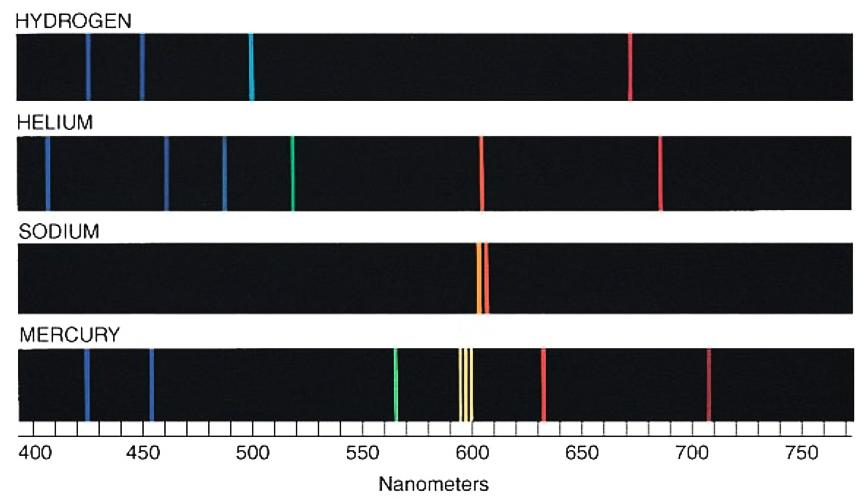
\includegraphics[width=10.5cm]{spectre.jpg}

\end{frame}

\appendix
\backupbegin
\begin{frame}[t]
	\frametitle{Questions?}
	\grid

	\pause
\end{frame}
\backupend

\end{document}
